\documentclass[a4paper, 12pt]{article}

% osnovni paketi za jezik in kodiranje znakov
\usepackage[slovene]{babel} 
\usepackage[utf8]{inputenc}
\usepackage[T1]{fontenc}
\usepackage{lmodern}

% dodatni paketi
\usepackage{amsmath, amssymb, amsthm}
% \usepackage[font=small, center]{caption}
\usepackage[hidelinks]{hyperref}
\usepackage{graphicx}
\usepackage{wrapfig}
\usepackage{float}     
\usepackage{geometry}
\usepackage[table]{xcolor} % http://ctan.org/pkg/xcolor
\usepackage{biblatex}
\addbibresource{literatura.bib}


\begin{document}

\begin{titlepage}
    \begin{center}
        \large
        Fakulteta za matematiko in fiziko\\
        Oddelek za matematiko \\
        \vspace{6cm}
        \Huge
        \textbf{Vizualizacija Kakeya-množice} \\
        \vspace{6cm}
        \large
        Terezija Krečič\\
        Pedagoška matematika, 5. letnik\\
        \vspace{1cm}
        Predmet: Matematika z računalnikom \\
        Mentor: Sergio Cabello\\
        \vspace{2cm}
        Ljubljana, 21. 5. 2024
    \end{center}
\end{titlepage}

\newpage


%%%%%%%%%%%%%%%%%%%%%%%%%%%%%%%%%%%%%%%%%%%%%%%%%%%%%%%%%%%%%%%%%

\section*{Uvod}

V tej projektni nalogi je bil cilj vizualizirati Kakeya-množico s pomočjo programa \href{https://ipe.otfried.org/}{Ipe}. Najprej sem morala sploh predelati problem, ki ga je zastavil Kakeya več kot sto let nazaj, poleg tega pa se še spoznati z novo programsko opremo.

V poročilu bom na kratko predstavila glavno vprašanje in eno strategijo, kako ga rešiti. Vse slike, ki so vključene zraven, sem ustvarila sama s pomočjo Geogebre in omenjenega orodja Ipe. 

Poročilo je izhaja iz Besicovitchevega članka~\cite{Besicovitch}, vendar sem nekaj delov poenostavila in predelala, saj sem se poskusila čimbolj izogniti upeljevanju novih oznak. Tako npr. pri poljubno majhni ploščini Pálovega spoja nisem strogo matematično zapisala, kakšen poljubno majhen kot moramo vzeti, in iz kota izpeljala formulo za ploščino spoja, temveč sem idejo zapisala le z besedami.

V poročilu bo najprej predstavljeno zastavljeno vprašanje, ki ga rešujemo, nato pa še en način generiranja take množice, ki ustreza pogoju iz vprašanja in nanj tudi odgovori.

\newpage

%%%%%%%%%%%%%%%%%%%%%%%%%%%%%%%%%%%%%%%%%%%%%%%%%%%%%%%%%%%%%%%%%

\section*{Kakeyev problem igle}

Japonski matematik Sōichi Kakeya je leta 1917 zastavil naslednje vprašanje, ki se ga je v kasnejšem času prijelo ime ``\emph{Kakeyev problem igle}''\footnote{orig. \emph{the Kakeya needle problem}, op. prev.}:

\vspace{0.2cm}
\begin{center}
    \textbf{Kolikšna je lahko najmanjša ploščina območja, znotraj katerega se daljica dolžine 1 zvezno obrne za 180°?}
\end{center}
\vspace{0.2cm}

\noindent Poglejmo si tri primere geometrijskih likov, ki ustrezajo pogoju iz vprašanja:

\begin{enumerate}
    \item krog s premerom 1 $ \rightarrow $ ploščina $ = \frac{\pi}{4} \doteq 0{,}79 $
    \item enakostranični trikotnik z višino 1 $ \rightarrow $ ploščina $ = \frac{1}{\sqrt{3}} \doteq 0{,}58 $
    \item deltoida\footnote{za konstrukcijo deltoide gl.~\cite{deltoida}, za animacijo obračanja igle znotraj nje pa~\cite{kakeya_wiki}}, včrtana v krog s premerom $ \frac{2}{3} $ $ \rightarrow $ ploščina $ = \frac{\pi}{8} \doteq 0{,}39 $
\end{enumerate}

\begin{figure}[h!]
    \centering
    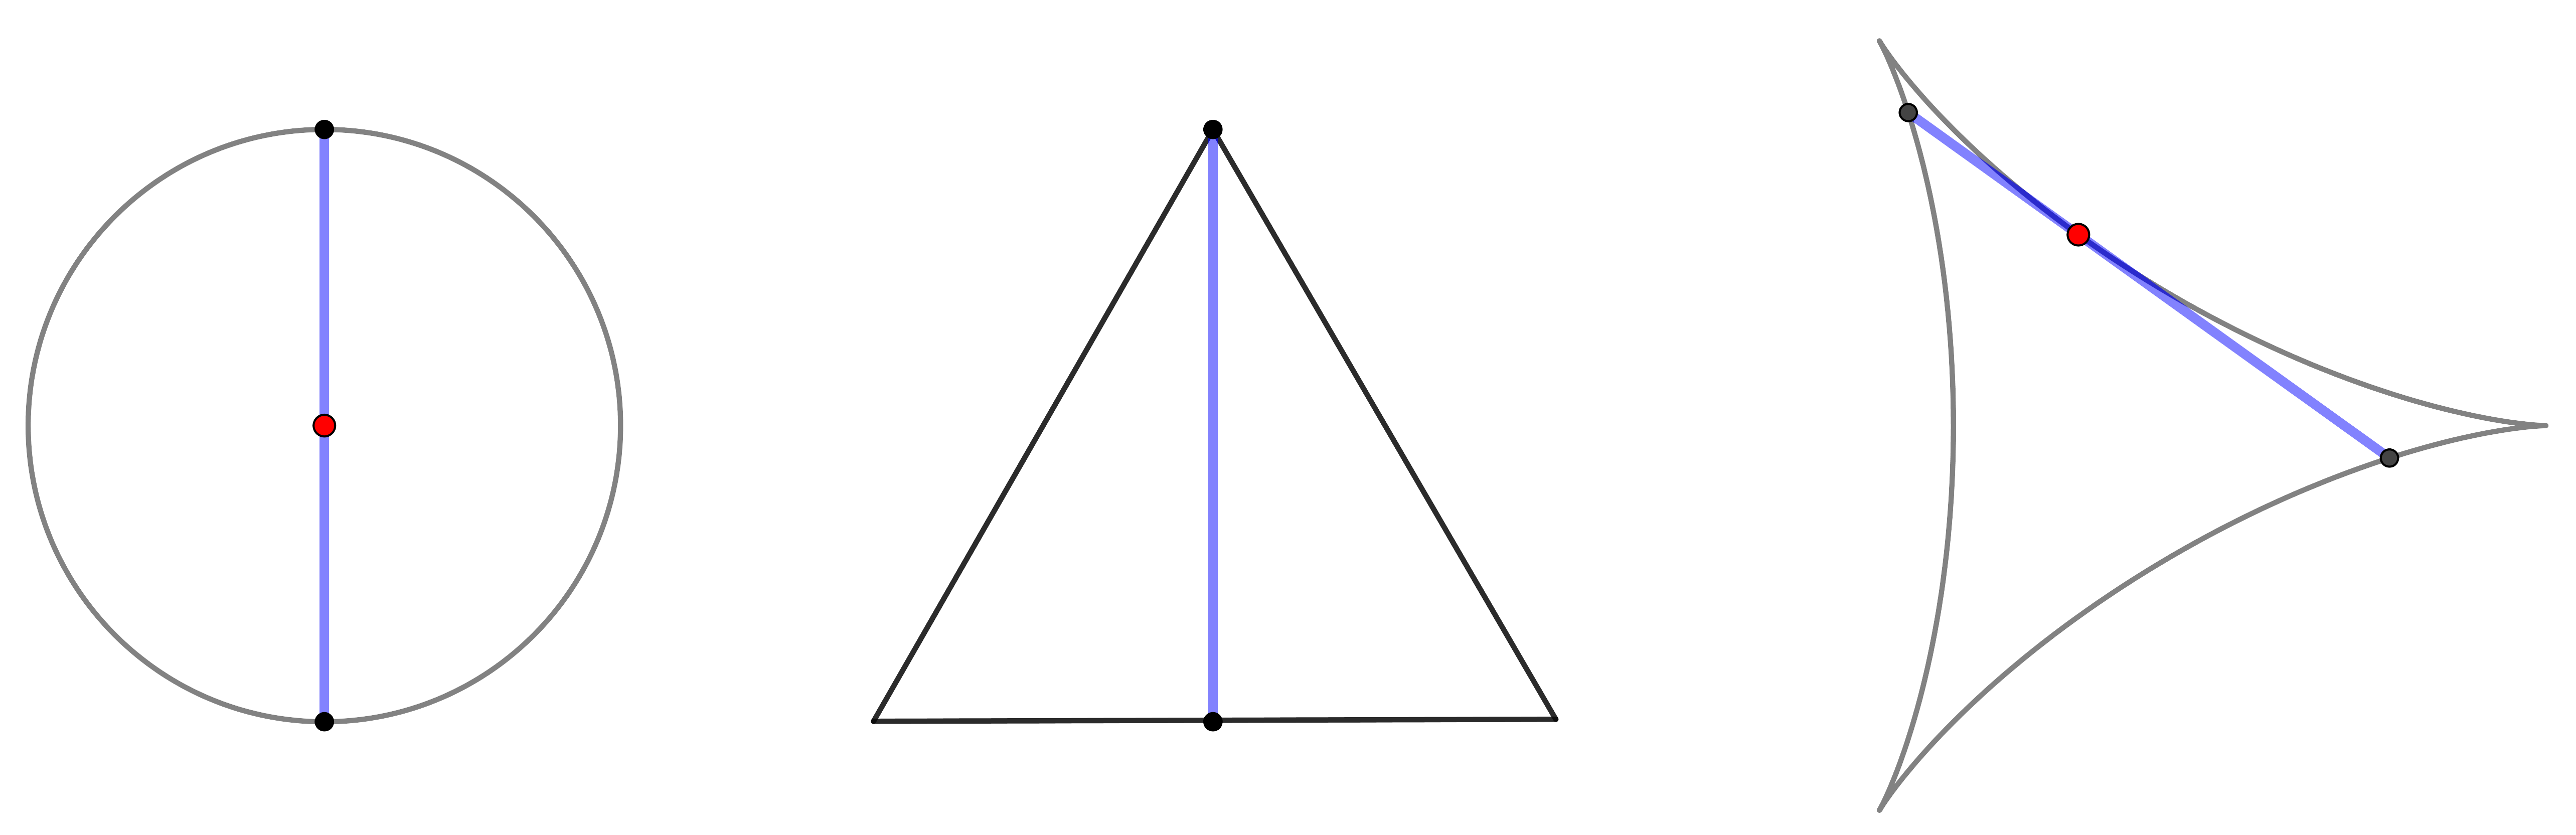
\includegraphics[width=0.8\textwidth]{geogebra_slike/prevelike_ploscine.png}
    \caption{Primeri, ki ustrezajo pogoju.}
    \label{primeri}
\end{figure}

Nekaj časa so verjeli, da je deltoida odgovor na vprašanje Kakeye, vendar je ruski matematik Abram Besicovitch uspel dokazati, da \textbf{spodnja meja za iskano ploščino \emph{ne} obstaja}. K enostavni konstrukciji primera takega lika je pripomogel nemški matematik Oskar Perron, svoj del pa je prispeval tudi madžarsko-danski matematik Gyula Pál.

%%%%%%%%%%%%%%%%%%%%%%%%%%%%%%%%%%%%%%%%%%%%%%%%%%%%%%%%%%%%%%%%%

\section*{Ideja za konstrukcijo}

Vzemimo enakokraki pravokotni trikotnik s katetama dolžine 2. Če v središče hipotenuze postavimo en konec enotske daljice, njen drugi konec opiše kot 180°, pri čemer daljica ves čas ostane znotraj lika. Trikotnik sicer ustreza pogoju iz vprašanja, vendar je njegova ploščina enaka 2 in večja od vseh treh zgornjih primerov.

Sedaj ga razdelimo na pol, kot kaže slika~\ref{trikotnik_razdelitev}, ter vsakega izmed delov (ki sta še vedno enakokraka pravokotna trikotnika, imenujmo ju ``\emph{osnovna trikotnika}'') še dodatno razdelimo na $ n $ manjših trikotnikov (imenujmo jih ``\emph{podtrikotniki}'') z osnovnico dolžine $ \frac{2}{n} $ in višino 1. Enotska daljica se tako obrne za 180°, ko se v enem krajišču zasuče čez vrh vsakega izmed podtrikotnikov in prehaja med njimi preko skupnih stranic.

\begin{figure}[h!]
    \centering
    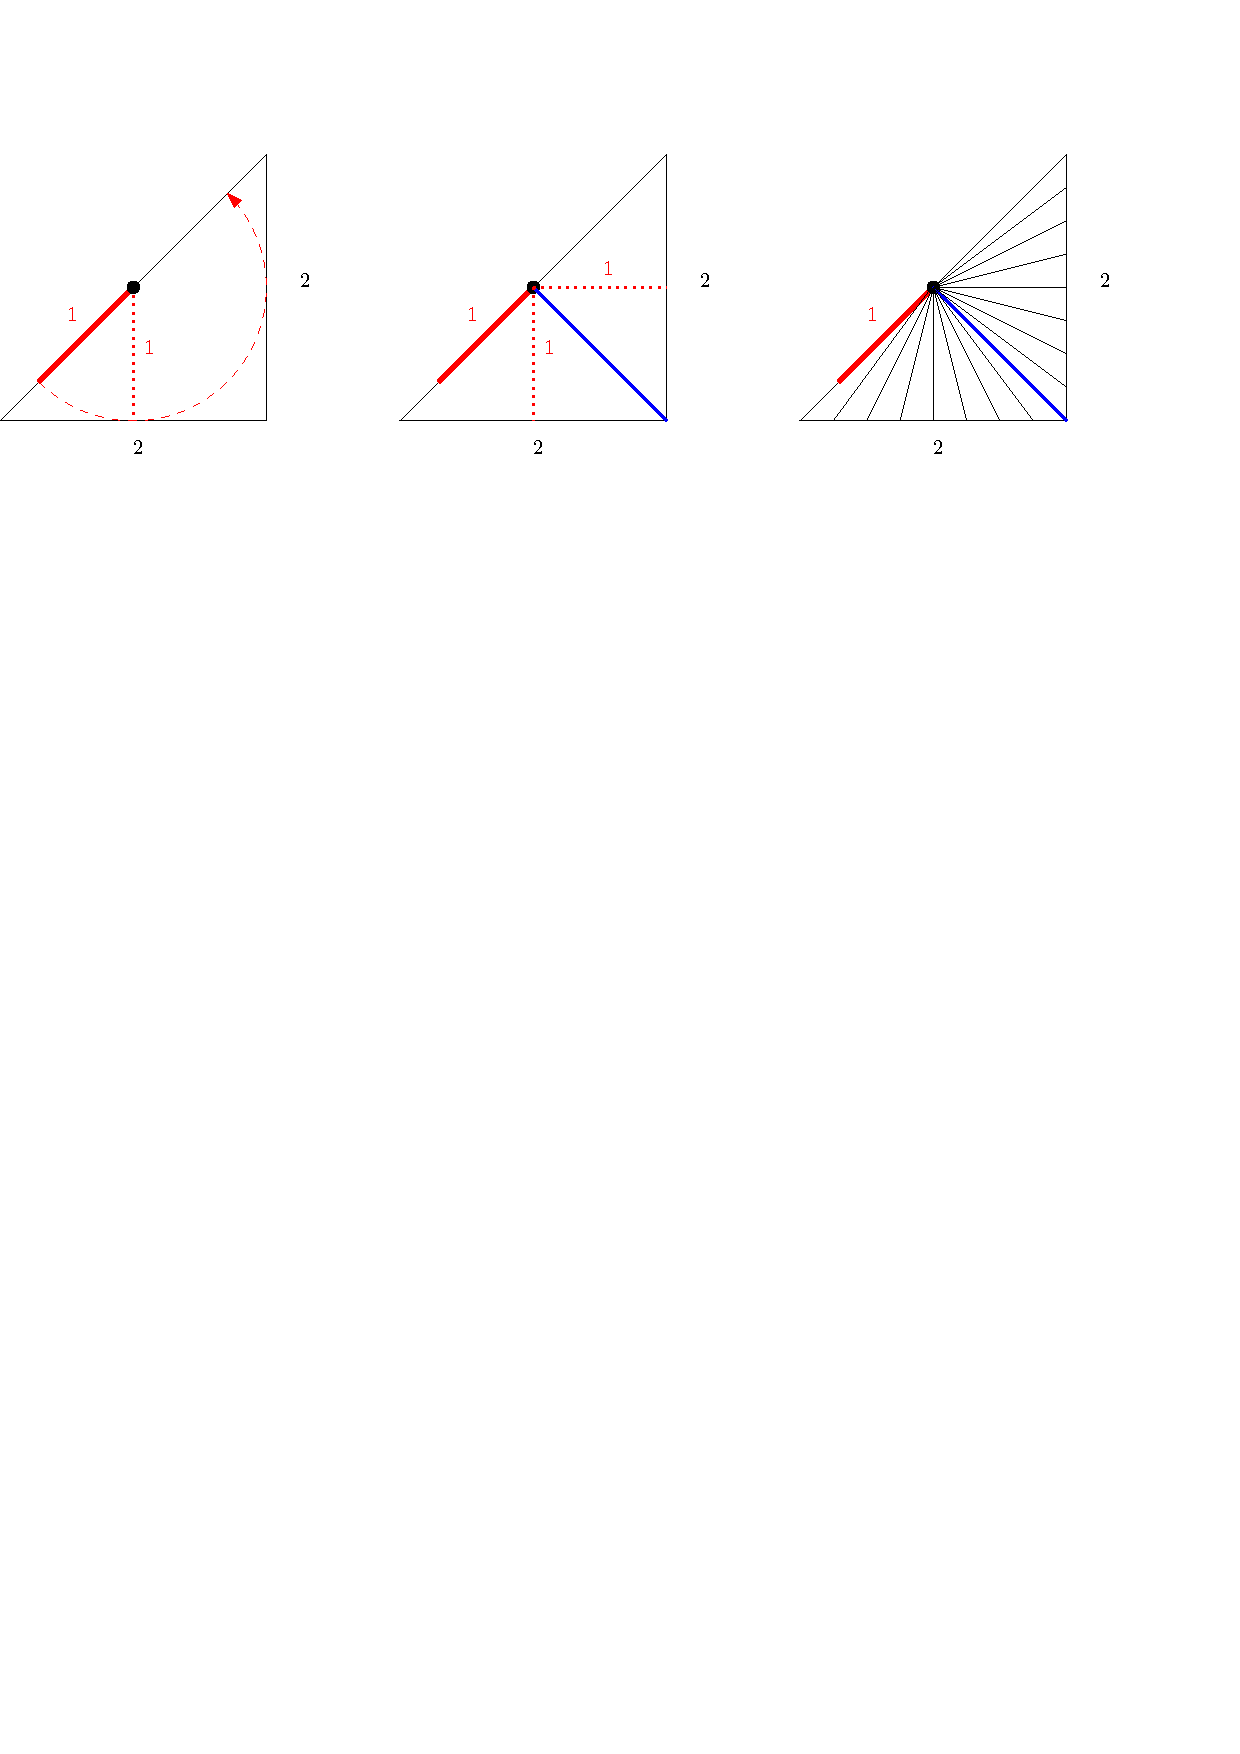
\includegraphics[width=\textwidth]{ipe_slike/trikotnik_razdelitev.pdf}
    \caption{Generiranje $ 2n $ podtrikotnikov z višino 1.}
    \label{trikotnik_razdelitev}
\end{figure}

\textbf{Ideja je, da teh $ 2n $ trikotnikov tako vzporedno premaknemo, da skupno prekritje tvori lik s poljubno majhno ploščino, ko $ n \to \infty $.}

Takoj opazimo, da se s translacijo podtrikotnikov prekine zvezen prehod enotske daljice iz enega podtrikotnika na drugega. Na sliki~\ref{preskok1} so narisane možne translacije sosednjih dveh podtrikotnikov. Skupne stranice so obarvane modro, enotska daljica pa z rdečo. Na levi ni spremembe in podtrikotnika se držita za skupno stranico, torej daljica zvezno preide iz levega podtrikotnika na desnega. V sredi imata podtrikotnika prazen presek, na desni pa se podtrikotnika prekrivata in pojavi se vprašanje, kako naj daljica iz modre stranice levega podtrikotnika preskoči na modro stranico desnega, kjer bi potem nadaljevala svoje vrtenje.

\begin{figure}[h!]
    \centering
    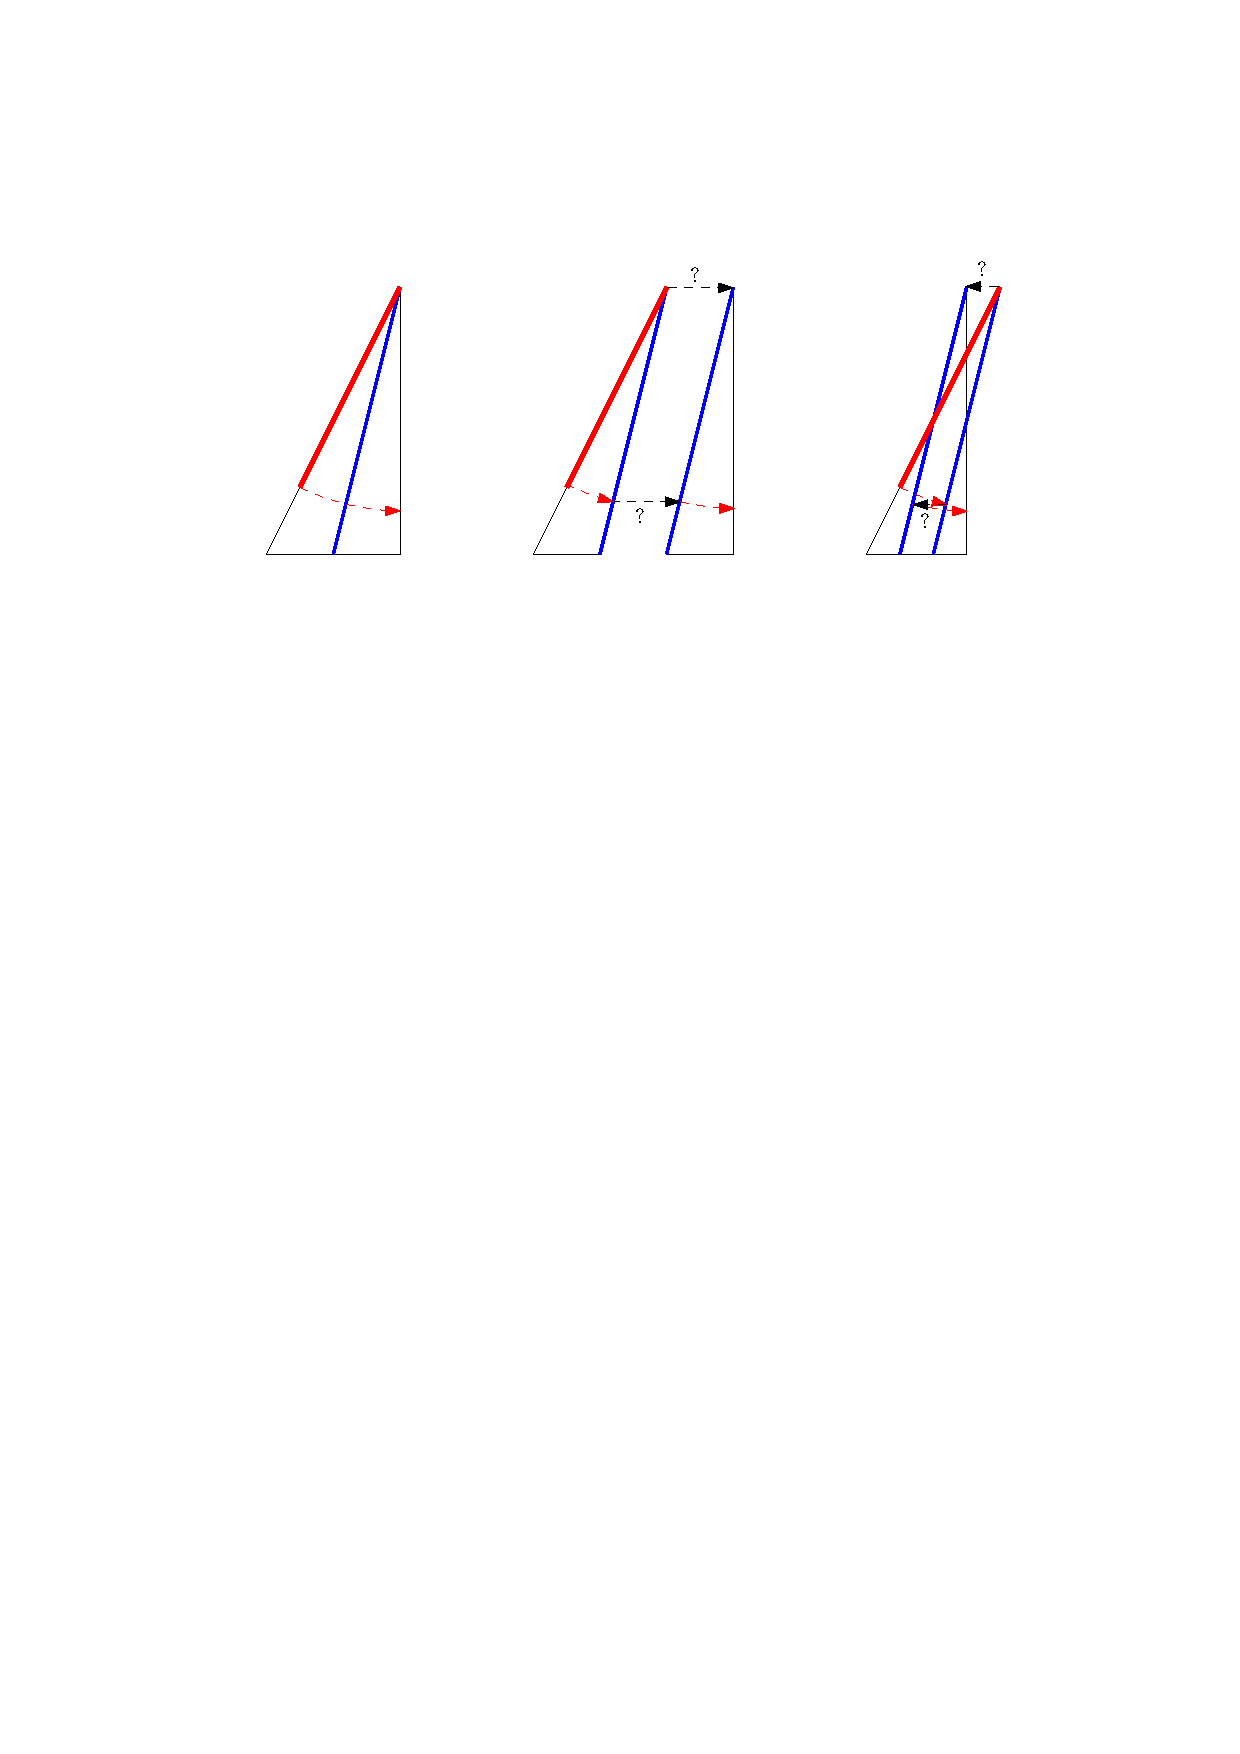
\includegraphics[width=0.7\textwidth]{ipe_slike/preskok1.pdf}
    \caption{Možne translacije sosednjih podtrikotnikov in vrtenje daljice skozi njiju}
    \label{preskok1}
\end{figure}

%%%%%%%%%%%%%%%%%%%%%%%%%%%%%%%%%%%%%%%%%%%%%%%%%%%%%%%%%%%%%%%%%

\section*{Preskok daljice med sosednjima trikotnikoma}

Pál je za preskakovanje daljice med dvema sosednjima podtrikotnikoma, ki se ne stikata več na skupni stranici (sredinski in desni primer na sliki~\ref{preskok1}), podal nadvse enostavno rešitev v naslednjih dveh korakih (gl. sliko~\ref{pal}):

\begin{enumerate}
    \item \textbf{Konstrukcija Pálovega spoja} (označen z zeleno): Nad prekrivajočima sosednjima podtrikotnikoma narišemo nosilki obeh modrih stranic, ki sta seveda vzporedni. Nato zarišemo daljico, ki ju povezuje, kot je narisano na sliki.
    \item \textbf{Gibanje po črki ``N''}: Ko se enotska daljica obrne v vrhu prvega podtrikotnika in pristane na modri stranici, jo pošljemo po prvi nosilki do začetka povezovalne daljice, kjer jo zavrtimo okoli zgornjega krajišča, da pristane na povezovalni daljici, nato jo premaknemo po tej daljici do vrha drugega podtrikotnika, jo zavrtimo v nasprotno smer, da pristane na drugi nosilki, po kateri jo nato potisnemo v drugi podtrikotnik.
\end{enumerate}

\begin{figure}[h!]
    \centering
    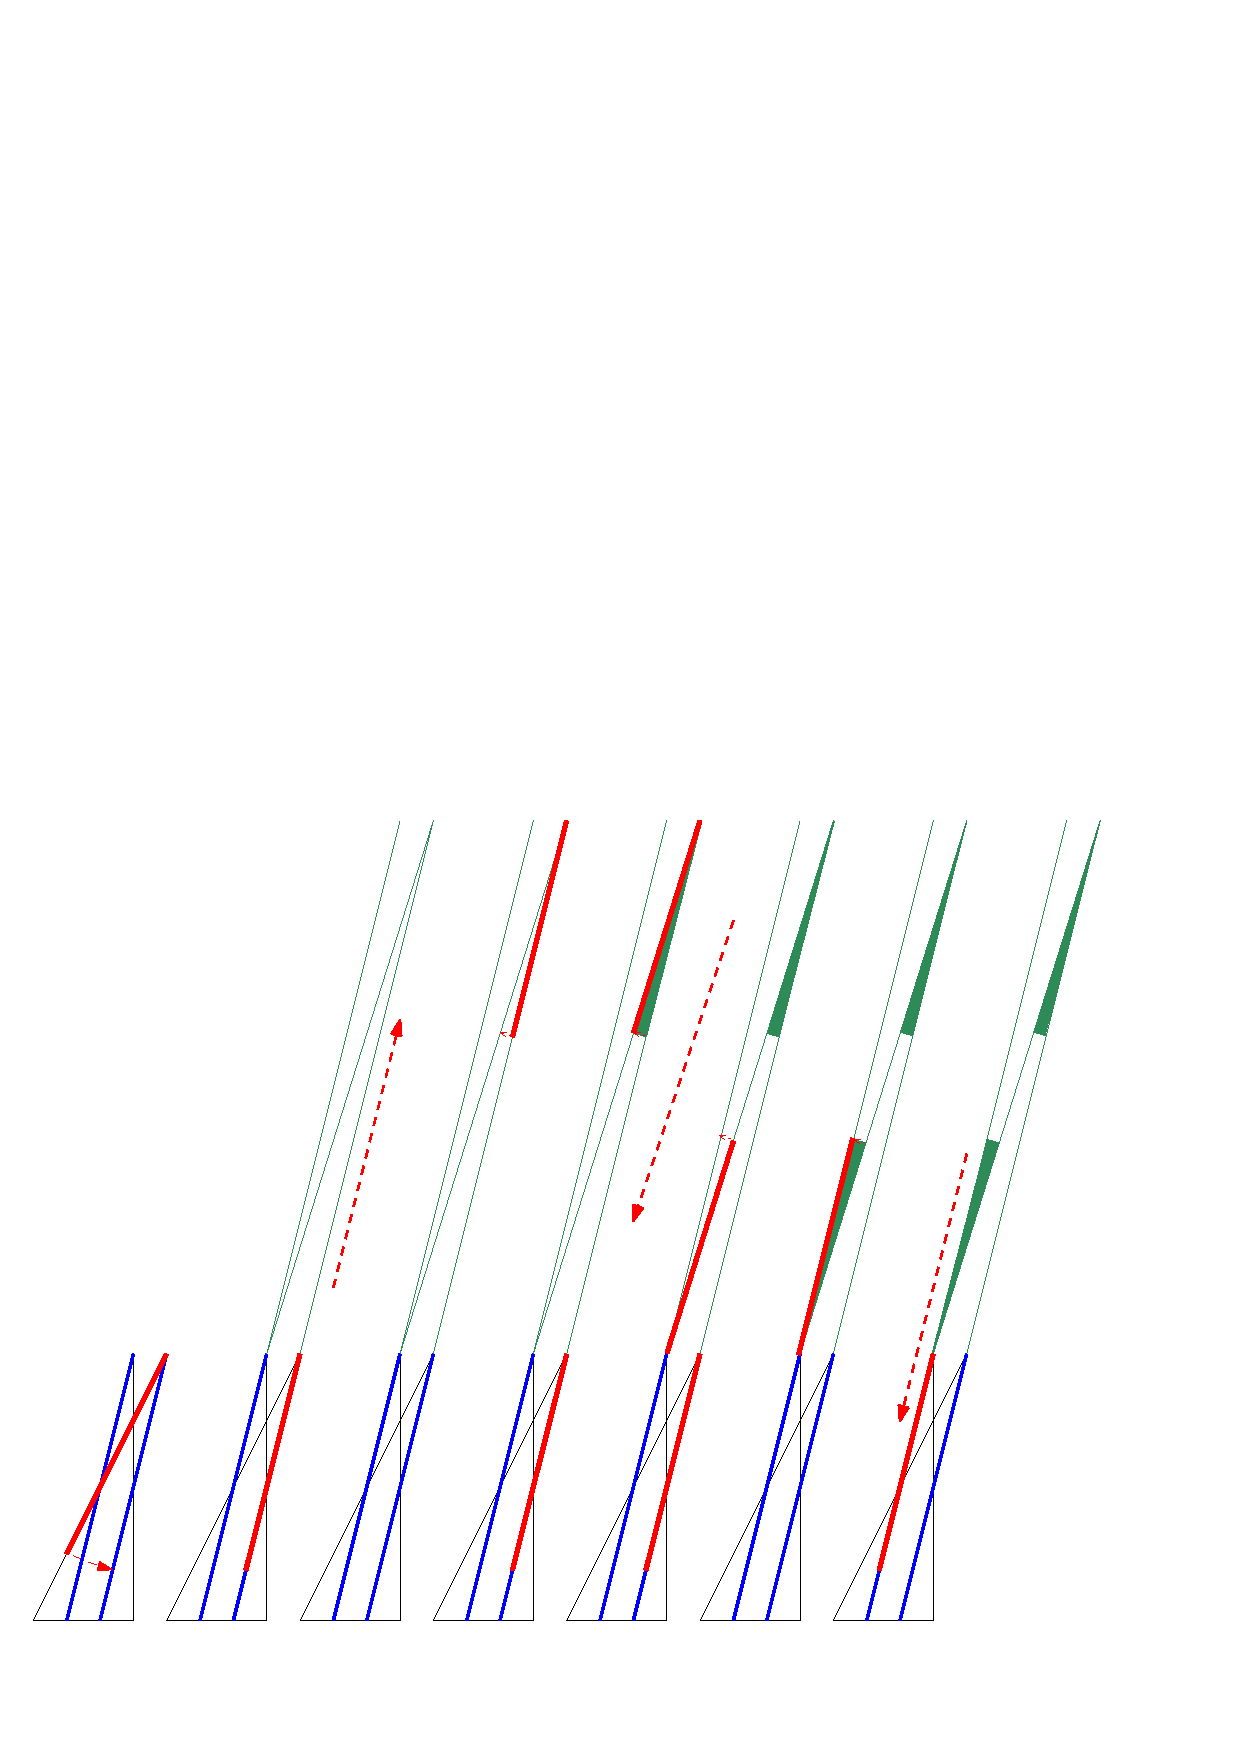
\includegraphics[width=\textwidth]{ipe_slike/pal.pdf}
    \caption{Preskok daljice preko Pálovega spoja}
    \label{pal}
\end{figure}

Smer enotske daljice se na ta način pri preskoku v sosednji podtrikotnik ohrani, daljica pa med tem prehodom (gibanjem po zelenem liku) opiše poljubno majhno ploščino, saj je kot vrtenja, če za zgornje krajišče povezovalne daljice izberemo poljubno oddaljeno točko na prvi nosilki, lahko poljubno majhen ter s tem tudi ploščina orisanega krožnega izseka, daljice pa k skupni ploščini tako ali tako ne prispevajo ničesar.

\textbf{Torej za vsak preskok enotske daljice med sosednjima podtrikotnikoma \emph{potrebujemo} (in znamo konstruirati) \emph{dodatno ploščino}, vendar je le-ta lahko \emph{poljubno majhna}.}

%%%%%%%%%%%%%%%%%%%%%%%%%%%%%%%%%%%%%%%%%%%%%%%%%%%%%%%%%%%%%%%%%

\section*{Perronovo drevo}

S Pálovimi spoji smo rešili težavo vzporednih translacij enotske daljice, pri čemer se je skupna ploščina lika povečala le za poljubno majhno vrednost.

Ostane nam še vprašanje, kako medsebojno prekriti podtrikotnike, da bo ploščina celotnega območja prekritja poljubno majhna, ko gre število podtrikotnikov proti neskončnosti. Tako bo skupaj s Pálovimi spoji ploščina območja, v katerem se enotska daljica obrne za 180°, poljubno majhna in s tem vprašanje Kakeye odgovorjeno.

\begin{wrapfigure}{r}{0.23\textwidth}
    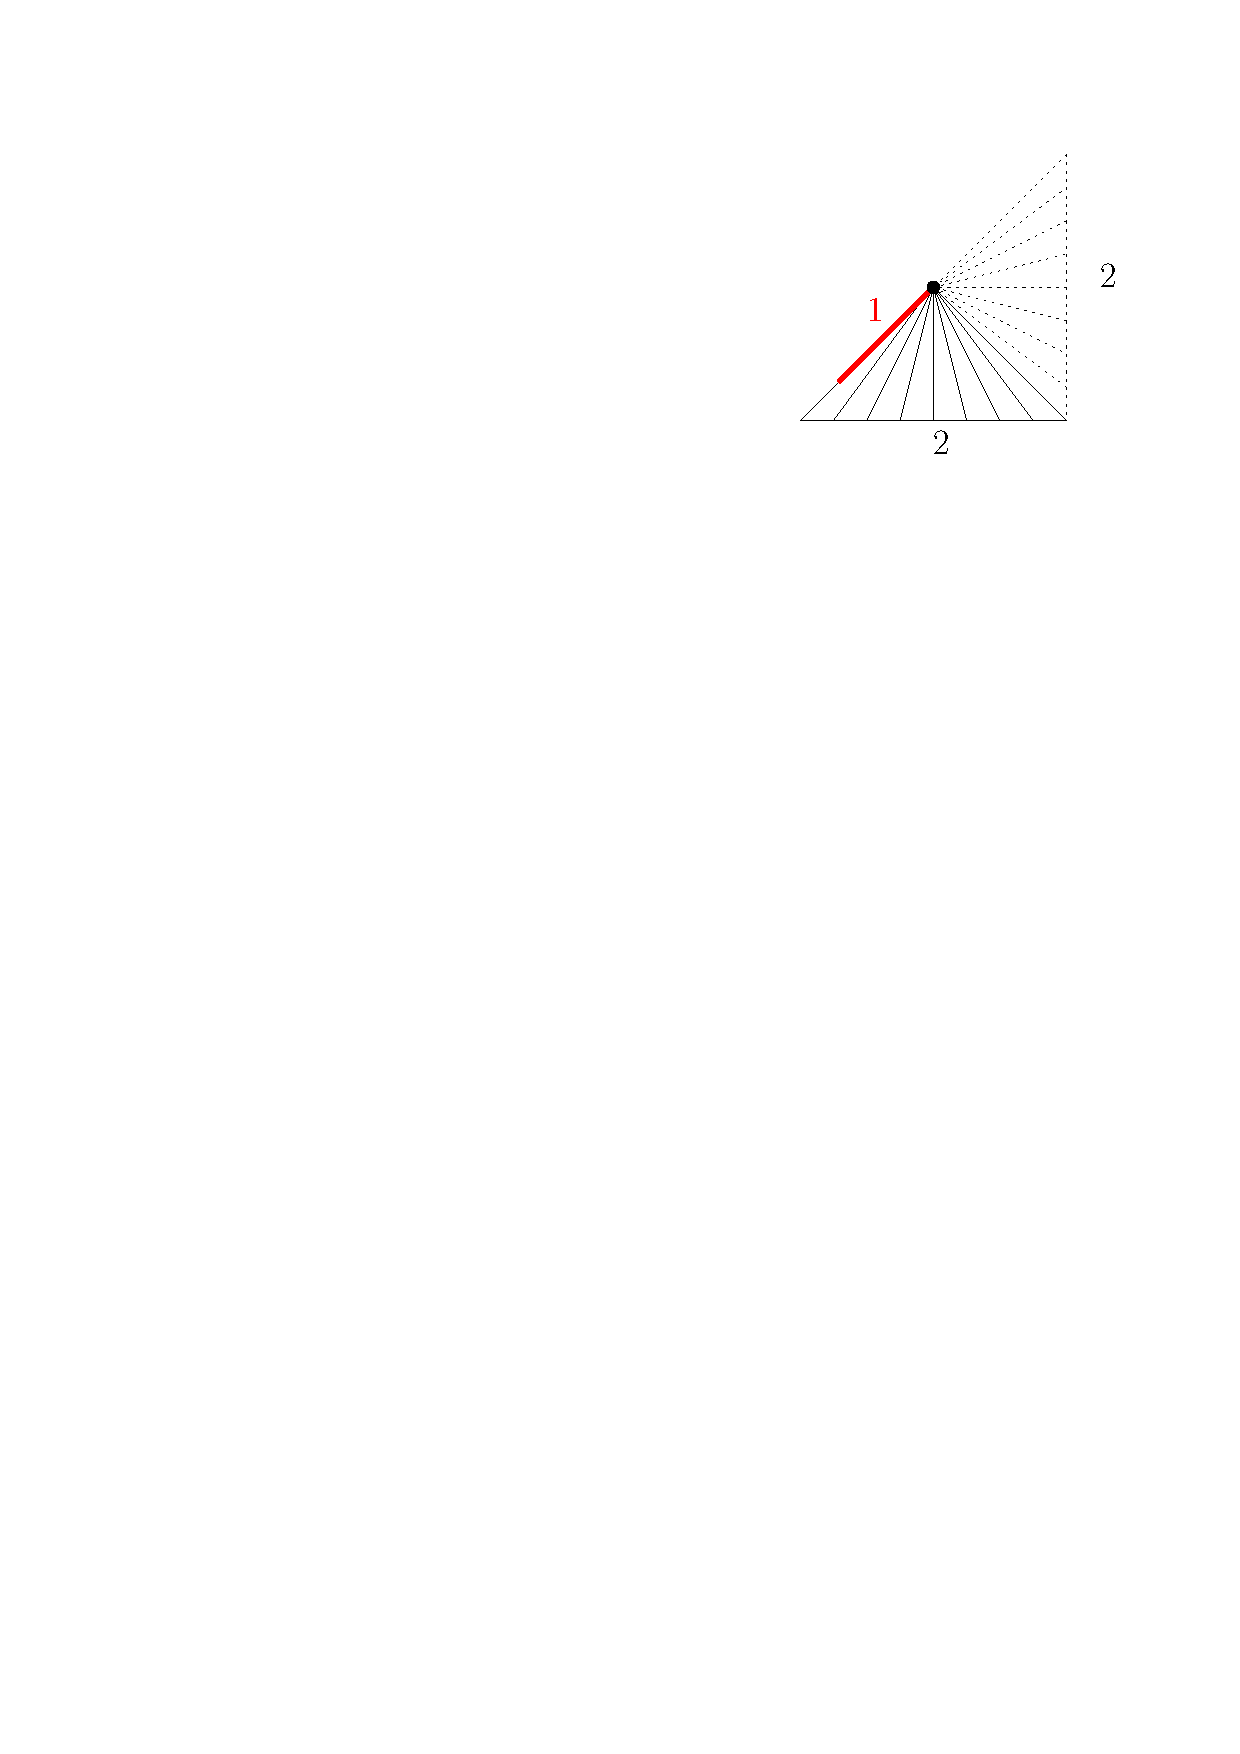
\includegraphics[width=0.9\linewidth]{ipe_slike/polovica_trikotnika.pdf}
\end{wrapfigure}

Perron je odkril zanimiv, a preprost in učinkovit način prekrivanja podtrikotnikov.

Spomnimo se, kako smo iz pravokotnega enakokratkega trikotnika dobili $ 2n $ manjših trikotnikov (slika~\ref{trikotnik_razdelitev}). Vzemimo spodnji osnovni trikotnik, ki je na desni označen z neprekinjeno črto, in na njem poglejmo konstrukcijo. Za drugi osnovni trikotnik, ki je pravokoten na prvega, bo postopek enak, le vse je obrnjeno za pravi kot v levo.

\begin{wrapfigure}{l}{0.45\textwidth}
    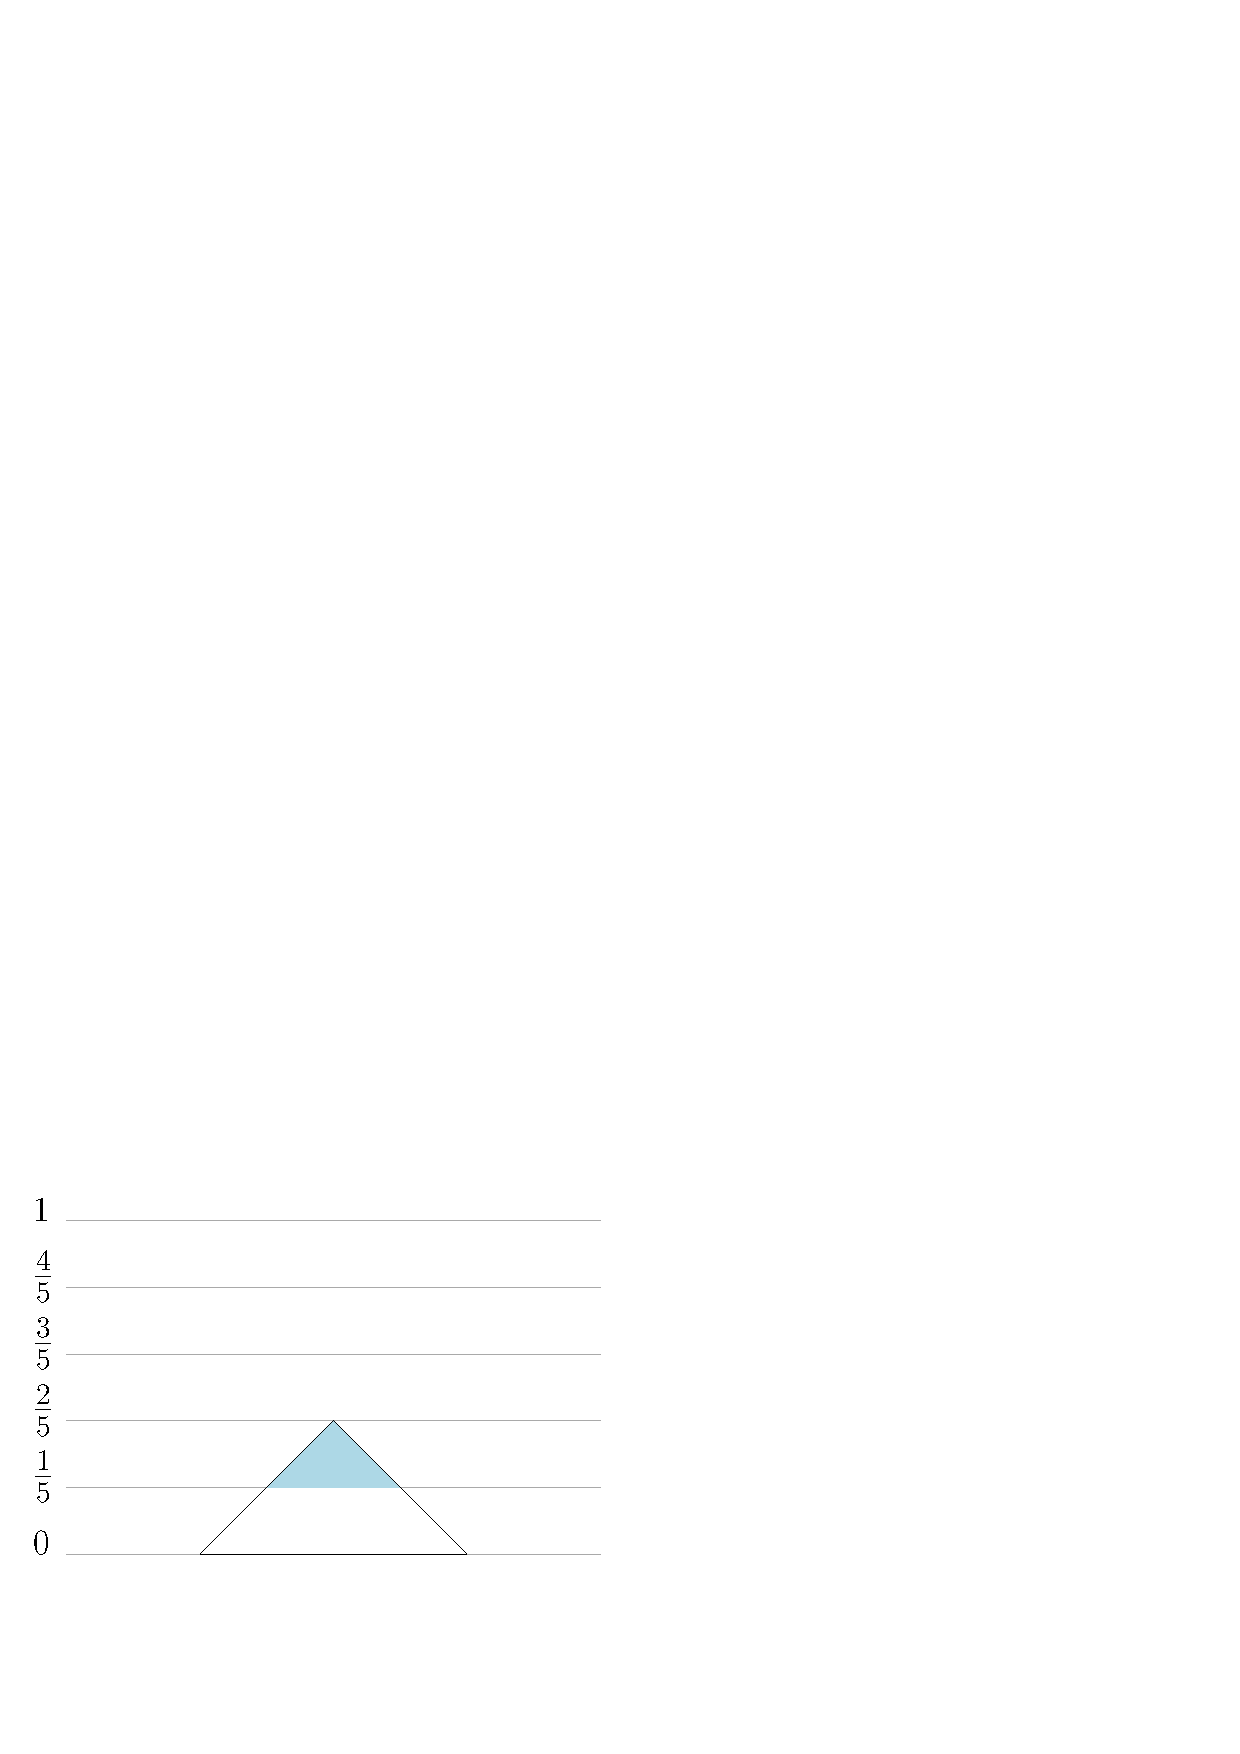
\includegraphics[width=0.9\linewidth]{ipe_slike/k_5.pdf}
    \caption{Koordinatni sistem ($ k = 5 $)}
    \label{sistem5}
\end{wrapfigure}

Pri konstrukciji bomo povečevali število podtrikotnikov, na katere je razdeljen osnovni trikotnik. Naj bo $ k \in \mathbb{N}, k \neq 1 $ (na slikah je $ k = 5 $) in naš koordinatni sistem tak, kot ga kaže slika~\ref{sistem5}: V vertikalni smeri smo dolžino 1 razdelili na $ k $ skladnih delov in dobili $ k $ ``nivojev''. Na sredo spodnje horizontalne črte položimo osnovnemu trikotniku podoben trikotnik z višino $ \frac{2}{k} $.

Definirajmo še \emph{vrh} -- to je vsak trikotnik z višino $ \frac{1}{k} $, ki v koordinatnem sistemu leži najvišje (na sliki ~\ref{sistem5} pobarvano modro).

Z naslednjim postopkom bomo zgenerirali osnovni trikotnik z višino 1, ki je razdeljen na medsebojno že premaknjenih $ 2^{k-2} $ podtrikotnikov: \emph{Nehorizontalne stranice vsakega vrha podaljšamo za en nivo navzgor. Zgornje krajišče vsake podaljšane daljice povežemo s spodnjim ogliščem vrha, ki leži na isti strani (torej se spustimo za dva nivoja navzdol). Tako originalen trikotnik dobi dva ``uhlja''.}

Postopek ponovimo za vsak nov vrh, dokler ne pridemo do nivoja 1, torej skupaj opravimo $ k-2 $ korakov. Postopek po avtorju imenujemo \textbf{brstenje Perronovega drevesa}.

\begin{figure}[h!]
    \centering
    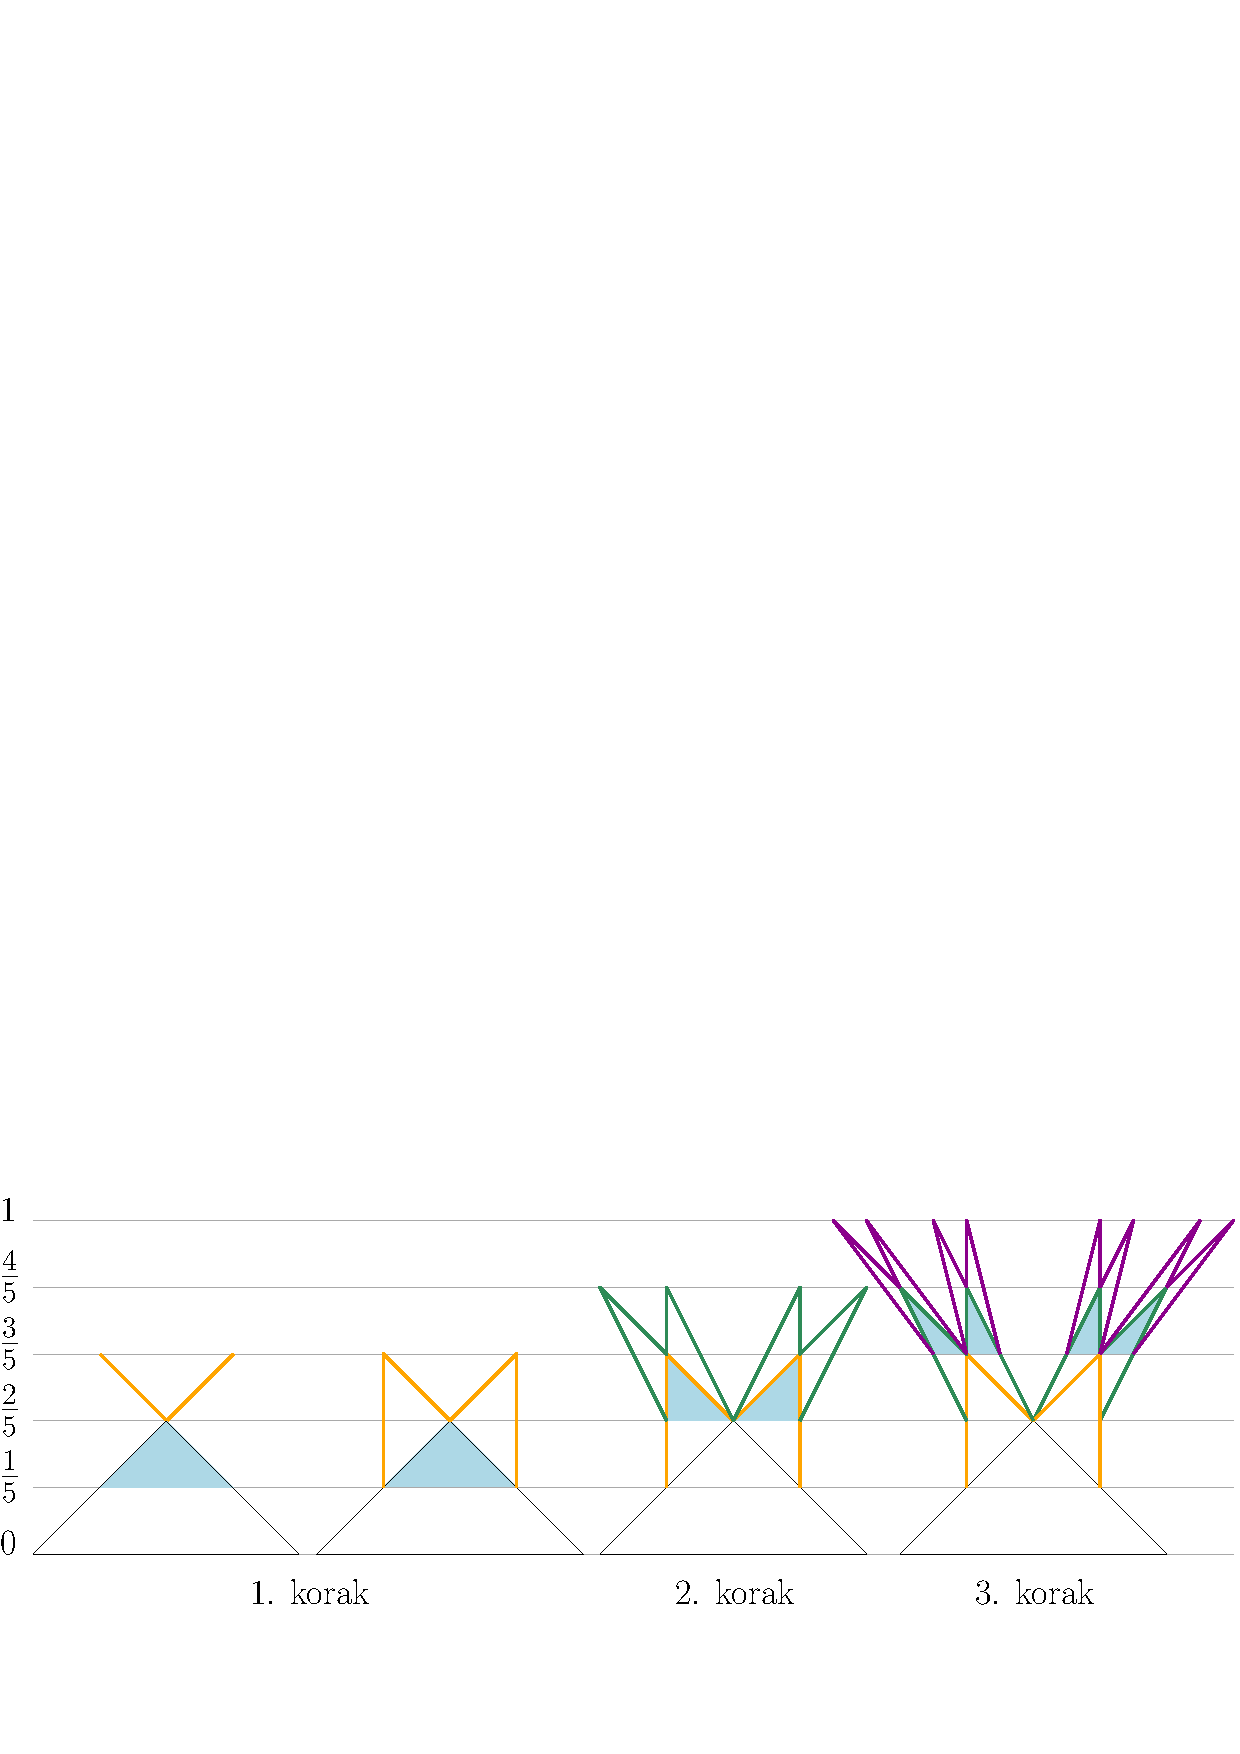
\includegraphics[width=\textwidth]{ipe_slike/koraki.pdf}
    \caption{Generiranje osnovnega trikotnika in podtrikotnikov za $ k = 5 $}
    \label{koraki}
\end{figure}

\noindent Sedaj moramo premisliti naslednje lastnosti te konstrukcije:

\begin{enumerate}
    \item Vsak vrh porodi skadna uhlja, ki imata enako ploščino kot taisti vrh.
    \item V $ l $-tem koraku ($ l = 1, 2, \ldots, k-2 $) dobimo $ 2^l $ prekrivajočih se podtrikotnikov, ki skupaj sestavijo osnovnemu trikotniku podoben trikotnik z višino $ \frac{l+2}{k} $.
    \item V vsakem koraku se nam skupna ploščina poveča za natanko dvakratno ploščino vrha, s katerim začnemo prvi korak, tj. za $ \frac{2}{k^2} $
    \item Skupna ploščina lika, ki ga dobimo na zadnjem koraku, je $ \frac{2}{k} $.
\end{enumerate}

%%%%%%%%%%%%%%%%%%%%%%%%%%%%%%%%%%%%%%%%%%%%%%%%%%%%%%%%%%%%%%%%%

\subsubsection*{Lastnost 1}

Poglejmo si uhlja, ki nastaneta na nekem vmesnem koraku iz enega od vrhov ((a) na sliki~\ref{uhlji}):

\begin{itemize}
    \item \emph{Ploščina uhljev} (b): Vsak trikotnik, sestavljen in vrha in enega izmed uhljev (označeno z zeleno), ima dvakratno ploščino vrha, saj je osnovnica skupna, višina pa dvakrat večja od višine vrha. Torej ima vsak uhelj enako ploščino kot vrh.
    \item \emph{Skladnost uhljev} (c): Zaradi podaljšanja stranic uhljev za en nivo navzgor imata uhlja dva para skladnih stranic ob sovršnem kotu, torej sta res skladna in sta njuni najdaljši stanici vzporedni.
\end{itemize}

\begin{figure}[h!]
    \centering
    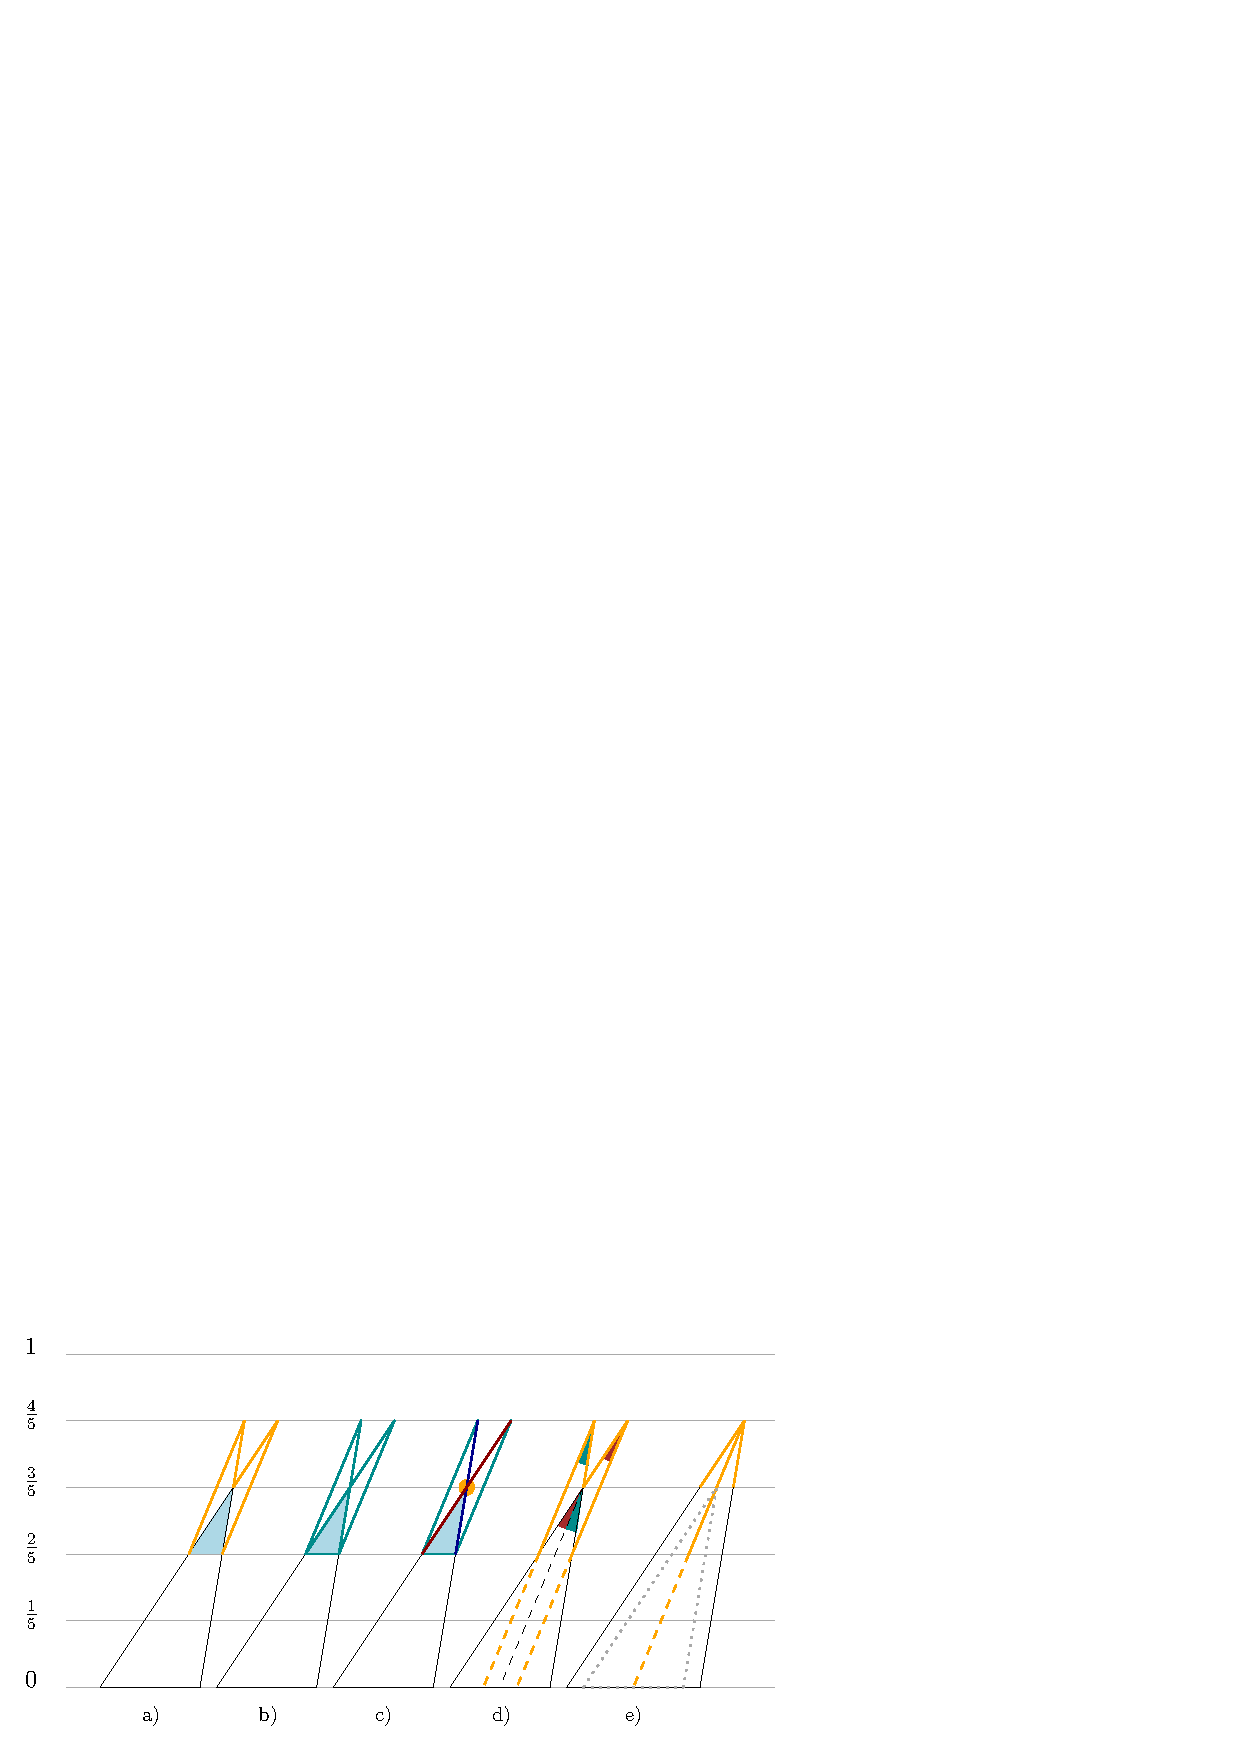
\includegraphics[width=0.9\textwidth]{ipe_slike/uhlji.pdf}
    \caption{Geometrijski dokaz lastnosti 1}
    \label{uhlji}
\end{figure}

Iz skladnosti sledi, sta tudi oranžni črtkani nosilki (d) vzporedni in smo dobili dva sosednja podtrikotnika, ki skupaj tvorita trikotnik, podoben prejšnjemu (e), le za $ \frac{1}{k} $ višji.

%%%%%%%%%%%%%%%%%%%%%%%%%%%%%%%%%%%%%%%%%%%%%%%%%%%%%%%%%%%%%%%%%

\subsubsection*{Lastnost 2}

Ker postopek začnemo s trikotnikom, ki je podoben osnovnemu trikotniku, ki ga želimo na koncu, in ker lastnost 1 pove, da na vsakem koraku iz trikotnika dobimo dva višja podtrikotnika, ki skupaj tvorita prejšnjemu podoben trikotnik, sledi, da v $ l $-tem koraku res dobimo $ 2^l $ podtrikotnikov, ki skupaj sestavijo ustrezno pomanjšan osnovni trikotnik. Njihova višina je $ \frac{l+2}{k} $, saj prvi korak začnemo na višini $ \frac{2}{k} $ in se vsakič dvignemo za $ \frac{1}{k} $ navzgor. V zadnjem koraku res dobimo $ 2^{k-2} $ podtrikotnikov.

%%%%%%%%%%%%%%%%%%%%%%%%%%%%%%%%%%%%%%%%%%%%%%%%%%%%%%%%%%%%%%%%%

\subsubsection*{Lastnost 3}

Zanima nas, za koliko se poveča skupna ploščina lika po vsakem koraku. Iz konstrukcije in podobnosti je razvidno, da v vsakem koraku novi vrhovi skupaj tvorijo ravno originalen vrh, s katerim smo začeli (slika~\ref{koraki}), vsak nov vrh pa je ploščinsko enak polovici uhlja. Torej se v vsakem koraku ploščina poveča za dvakratno  skupno ploščino novih vrhov, torej za dvakratno ploščino originalnega vrha, tj. za $ 2 \cdot \frac{2}{k} \frac{1}{k} \frac{1}{2} = \frac{2}{k^2} $.

%%%%%%%%%%%%%%%%%%%%%%%%%%%%%%%%%%%%%%%%%%%%%%%%%%%%%%%%%%%%%%%%%

\subsubsection*{Lastnost 4}

Skupna ploščina je tako sestavljena iz ploščine prvotnega trikotnika z višino $ \frac{2}{k} $ in iz na vsakem koraku dodanih ploščin. Opravili smo $ (k-2) $ korakov, torej je skupna ploščina Perronovega drevesa za izbrani $ k $ enaka

\begin{equation*}
    \frac{4}{k} \cdot \frac{2}{k} \cdot \frac{1}{2} + (k -2) \cdot \frac{2}{k^2} = \frac{2}{k}.
\end{equation*}

S to konstrukcijo smo prišli do rešitve, ki jo je našel že Besicovitch, saj večji kot je $ k $, manjša je skupna ploščina lika in posledično lahko dobimo poljubno majhno ploščino.



%%%%%%%%%%%%%%%%%%%%%%%%%%%%%%%%%%%%%%%%%%%%%%%%%%%%%%%%%%%%%%%%%
\newpage

\section*{Povzetek rezultatov}

Osnovni trikotnik z višino 1 smo razdelili na $ n = 2^{k-2} $ podtrikotnikov in jih medseboj tako prekrili, da smo dobili Perronovo drevo. Ploščina dobljenega lika je $ \frac{2}{k} $. Za prehod enotske daljice med sosednjimi podtrikotnikom potrebujemo še $ n-1 $ Pálovih spojev, ki pa skupaj doprinesejo poljubno majhno ploščino.

Postopek ponovimo še na drugem osnovnem trikotniku, ki je pravokoten na prvega. Lika združimo, kot kaže slika~\ref{zdruzitev}, in dobimo skupno ploščino največ $ \frac{4}{k} $ plus poljubno majhno vrednost, ki pride iz $ 2n - 1 $ Pálovih spojev (dodali smo še spoj za prehod enotske daljice iz prvega osnovnega trikotnika v drugega). Ko povečujemo $ k $ (in s tem tudi $ n $), gre skupna ploščina proti 0.

Zaključimo z odgovorom na vprašanje Kakeye -- \textbf{ploščina območja, znotraj katerega se enotska daljica zvezno obrne za 180°, je lahko poljubno majhna}.

%%%%%%%%%%%%%%%%%%%%%%%%%%%%%%%%%%%%%%%%%%%%%%%%%%%%%%%%%%%%%%%%%
\section*{Zaključek}

Lahko bi vzeli tudi enakostraničen trikotnik (vrh s 60°) in postopek izvedli 3x namesto 2x. Kakršenkoli trikotnik bi bil vredu, najbolj tak, kjer kot v vrhu deli 180°.

Besicovitch set -- množica, ki vsebuje enotsko daljico v vsaki smeri (ni pa nujno, da se lahko zvezno obrne)

%%%%%%%%%%%%%%%%%%%%%%%%%%%%%%%%%%%%%%%%%%%%%%%%%%%%%%%%%%%%%%%%%
\newpage
% \nocite{*}      % navede tudi vire, ki jih ne citiras
\printbibliography[heading=bibintoc, title={Literatura}]

%%%%%%%%%%%%%%%%%%%%%%%%%%%%%%%%%%%%%%%%%%%%%%%%%%%%%%%%%%%%%%%%%

\end{document}